%!TEX root = thesis.tex

%:-------------------------- Preamble -----------------------

\documentclass[final,10pt]{../../uit-thesis}

% Lorem ipsum
\usepackage{lipsum}

% Make glossaries
\makeglossaries

\begin{document}

%:-------------------------- Frontpage ------------------------

\thesisfaculty{Faculty or department}
\title{Title of the master thesis}
\thesissubtitle{Subtitle}
\author{Name of author}
\thesisprogramme{Master thesis in Computer Science… Month 20xx}

% (Optional) Set frontpage image
% \renewcommand\ThesisFrontpageImagePath{748443511_095ae916df_o.jpg}

\maketitle

%:-------------------------- Frontmatter -----------------------
\frontmatter

% Create toc, list of figures and list of tables. Remove if any of these are not desired
\tableofcontents

\newacronym{api}{API}{application programming interface}

\printglossaries
\addcontentsline{toc}{chapter}{\acronymname}

%:-------------------------- Mainmatter -----------------------
\mainmatter

\chapter{Introduction}
\lipsum[1]
\lipsum[1]
\lipsum[1-7]

We can use the \ac{api} to do stuff!

Referencing figure \ref{fig:ex} to test link.

\begin{figure}\label{fig:ex}
\centering
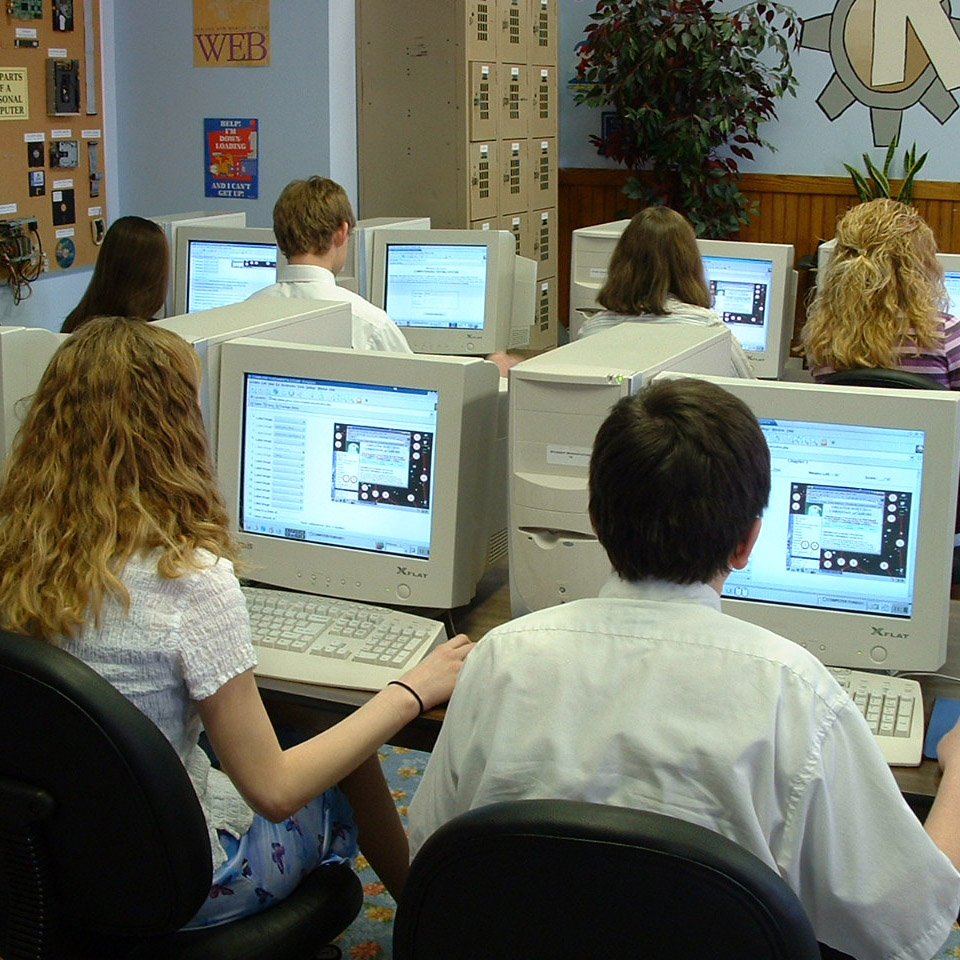
\includegraphics[scale=0.1]{748443511_095ae916df_o.jpg}
\caption{Figure link should point to top of figure.}
\end{figure}

\chapter{Design}
\lipsum[8-10]

\backmatter

\end{document}

